\chapter{Przetwarzanie heterogeniczne}\label{cha:hpo}

%---------------------------------------------------------------------------

\section{Wprowadzenie}\label{sec:wprowadzenie}


Lata 50-te XX wieku były przełomowym okresem w dziedzinie elektronicznego przetwarzania danych. Opracowana w 1945 roku Architekura von Neumana [16] pozwoliła na uruchomienie pierwszych komputerów ogólnego przeznaczenia. Mimo, że Architektura Harwardzka [17] została opracowana 6 lat wcześniej, Architektura von Neumana była łatwiejsza w implementacji przez przechowywanie danych wraz z programem na jednej wspólnej pamięci. Pierwszym komputerem opartym na pomyśle Neumana, który wykonywał instrukcje zapisane w fizycznej pamięci , był powstały w 1948 roku Small-Scale Experimental Machine. Był on bazą do rozwijania kolejnych urządzeń i tak w 1949 roku powstał EDSAC (akronim od ang. Electronic Delay Storage Automatic Calculator). Został uznany jako  pierwszy komputer wykorzystywany w praktyce do obliczeń naukowych. EDSAC rozbudowany był o dodatkowe układy peryferyjne. W celu odczytu danych zastosowano w nim dalekopis – aparat drukujący dane w postaci alfanumerycznej. Skonstruowanie komputerów zerowej, pierwszej i drugiej generacji znacznie rozwinęło moc obliczeniową tych urządzeń. W dalszym ciągu jednak stosowano niewygodne formy prezentacji danych – wyświetlacze złożone z szeregu lamp, perforowane karty. W 1975 roku, w jednym z pierwszych komputerów osobistych IBM 5100, zastosowano kineskopowy wyświetlacz, który mógł wyświetlać 16 linii po 64 znaków. 6 lat później , w kolejnym modelu IBM 5150, wprowadzono możliwość instalacji kart rozszerzeń ISA. Zastosowano w nim pierwszą kartę graficzną Monochrome Display Adapter (MDA). Rozpoczęło to rozwój peryferyjnych układów komputera, które stały się niezależnymi platformami z własnym procesorem i pamięcią. Początkowo karty graficzne były w stanie wyświetlać jedynie znaki alfanumeryczne przechowywane w pamięci karty. Kolejne generacje kart pozwalały na rysowanie obrazów przy użyciu pojedynczych pikseli, a nowoczesne układy graficzne pozwalały na akcelerację 2D i 3D, korzystając z wbudowanych funkcji do generowania obrazu. W najnowszych procesorach grafiki umożliwiono użytkownikowi zaprogramowanie ich w dowolny sposób. Charakterystyka obliczeń przy przetwarzaniu obrazów wymusiła architekturę procesorów graficznych w postaci dużej ilości jednakowych jednostek ALU (ang. Arithmetic Logic Units), potrafiących wykonać równolegle wiele prostych operacji (Rys. 3.1.).
\begin{figure}[h]
        \centering
                \centering
                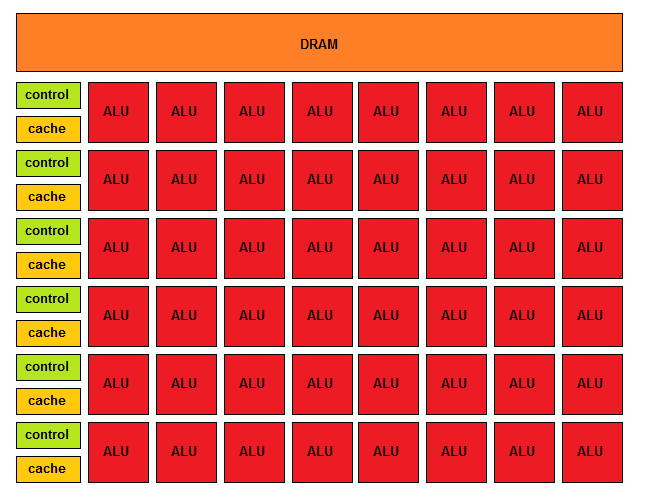
\includegraphics[width=12cm]{rys7}
	\caption{Architektura procesora GPU.}
\end{figure}
Taka budowa kart graficznych pozwoliła na wykorzystanie ich nie tylko do obliczeń związanych z generowaniem grafiki, ale także innych obliczeń przetwarzania danych , co doprowadziło do powstania kart ogólnego przeznaczenia (GPGPU).



%---------------------------------------------------------------------------

\section{Heterogeniczne platformy obliczeniowe}\label{sec:hetero}

Początkowo GPGPU były wykorzystywane do zaawansowanego generowania grafiki. Dążenie do realizmu w grach komputerowych rozwinęło karty graficzne o algorytmy wymagające przetwarzania równoległego, takie jak shading [18] czy ray-tracing [19]. W celu odciążenia procesora od złożonych obliczeń, na kartach graficznych zaczęto implementować fizykę obiektów – obliczenia związane z mechaniką klasyczną, symulacje zachowania cieczy, zachowania układów ciągłych i inne efekty cząsteczkowe. Dla ułatwienia programistom wykorzystania możliwości GPGPU, NVIDIA w 2007 roku wprowadza platformę CUDA. Jest to środowisko programistyczne i biblioteka umożliwiająca wykorzystanie kart graficznych produkowanych przez firmę NVIDIA. Umożliwia ona pisanie kodu opartego na C/C++ wykonywanego na procesorze karty i mającego bezpośredni dostęp do jej pamięci. Ułatwienie implementacji algorytmów na GPGPU rozwinęło wykorzystywanie tych kart w różnych dziedzinach naukowych, takich jak kryptografia, fizyka kwantowa, ekonomia czy medycyna. Wykonywanie  skomplikowanych obliczeń przy użyciu CUDA stało się powszechne na komputerach domowych, ale było ograniczone przez wymagania sprzętowe. 2 lata po wprowadzeniu CUDA firma Apple Inc wprowadza OpenCL (ang. Open Computing Language). W przeciwieństwie do produktu NVIDA, OpenCL umożliwia pisanie programów na heterogeniczne platformy – układy złożone z różnego rodzaju procesorów. Daje to możliwość pisania aplikacji na komputery z układami większości popularnych producentów, lub dowolne układy złożone z różnych procesorów (m. in. CPU, GPU, DSP, FPGA), oraz zapewnia przenośność programów.

%---------------------------------------------------------------------------

\section{Modele obliczeń równoległych}\label{sec:Paralellism}

Obliczenia równoległe to typ obliczeń komputerowych, w których wiele instrukcji wykonywanych jest jednocześnie [Gottlieb, Allan; Almasi, George S. (1989). Highly parallel computing. Redwood City, Calif.: Benjamin/Cummings. ISBN 978-0-8053-0177-9.]. Złożone problemy często mogą być rozłożone na mniejsze zadania, które mogą być wykonywane w tym samym czasie. Daje to możliwość szybszego rozwiązywania problemów bez zwiększania częstotliwości taktowania procesora. W uproszczeniu energia wydzielana przez procesor, a w większości ciepło, wzrasta wraz z kwadratem częstotliwości taktowania. Ze względu na te fizyczne ograniczenia procesora wielordzeniowe procesory i obliczenia równoległe stały się dominującym paradygmatem architektury komputerów.

Obliczenia równoległe dzielą się na cztery różne modele:

- równoległość bitów

- równoległość instrukcji

- równoległość danych

- równoległość zadań.

Modele obliczeń równoległych mogą być implementowane oddzielnie, lub w połączeniu ze sobą.

\subsection{Równoległość bitów}\label{sec:bitp}

Równoległość na poziomie bitów jest modelem przetwarzania równoległego opartym na zwiększaniu ilości bitów w pojedyńczym słowie procesora. Zwiększenie pojemności słowa zmniejsza liczbę instrukcji, które procesor musi wykonać, aby wykonać operację na zmiennych, których rozmiary są większe niż długość słowa.
Początkowo komputery opierały się na jednobitowych procesorach. Pierwszym nieszeregowym komputerem był 16-bitowy Whirlwind z 1951 roku. Obecnie w komputerach osobistych funkcjonuje standard 32 i 64-bitowych architektur procesorów i systemów operacyjnych. Większa szerokość słowa wymagałaby znacznie większej zewnętrznej szyny danych, co jest kosztowne do wykonania przy obecnych procesach technologicznych. 64-bitowe słowo w większości jest wystarczające do  procesowania zmiennych wykorzystywanych na komputerach osobistych. Przy złożonych obliczeniach inżynierskich duże dane przechowuje się na kilku zmiennych i przetwarza przy użyciu kilku instrukcji procesora.

\subsection{Równoległość instrukcji}\label{sec:instp}

Równoległość na poziomie instrukcji jest oparta na równoległym wykorzystaniu kilku jednostek wykonawczych procesora. Większość procesorów składa się z kilku jednostek arytmetyczno-logicznych ALU, odpowiadających za wykonywanie operacji arytmetycznych i logicznych przez procesor, oraz kilku jednostek zmiennoprzecinkowych FPU, odpowiadających za wykonywanie operacji arytmetycznych na liczbach zmiennoprzecinkowych. Wszystkie jednostki ALU i FPU mogą wykonywać operacje równolegle. Przykładowo, w poniższym kodzie (Kod ...), operacja z linijki 4 może być wykonana na jednostce ALU, a operacja z linijki 5 na jednostce FPU. Wykorzystując równoległość na poziomie instrukcji obie operacje mogą być wykonane przy użyciu jednej instrukcji procesora.

\begin{program}
\caption{Plik wejściowy programu}
\begin{lstlisting}
float a = 1.0, b = 2.0, c;
int x = 1, y = 2, z, w;

c = a + b;
z = z * y;
\end{lstlisting}
\end{program}

W zależności od architektury komputera, rozdzielenie operacji na jednostki wykonawcze procesora może być wykonane dynamicznie w trakcie wykonywania programu, lub statycznie na poziomie kompilacji. Dynamicznie ustawiana równoległość instrukcji wykorzystywana jest w powszechnie dostępnych procesorach CPU. Zwiększa ona szybkość wykonywania programu i odciąża programistę i kompilator od procesu rozdzielenia instrukcji. Rozmieszczenie instrukcji na etapie kompilacji wykorzystywane jest w procesorach DSP i GPU. Pozwala to optymalizację kodu przed jego wykonaniem i obliczenie dokładnego czasu w jakim program będzie się wykonywał.  

\subsection{Równoległość danych}\label{sec:datap}

Równoległość na poziomie danych wykorzystywana jest przy obliczeniach na dużych zbiorach danych, gdzie obliczenia dla pojedyńczych danych są od siebie niezależne. W tym modelu zbiór danych dzielony jest na mniejsze zbiory i definiowany jest zestaw zadań, które zostaną wykonane na pojedyńczego zbioru. Mniejsze zbiory danych wysyłane są do oddzielnych jednostek sterujących, które wykonują na nich równolegle zdefinowany zestaw zadań. Równoległość danych jest najwydajniejsza dla dużych zbiorów podobnych danych (np. wektory, macierze), dla prostych operacji, takich mnożenie macierzy, transformata Fouriera. Szybkość wykonywania programu opartego na tym modelu zależy od ilości jednostek sterujących, dlatego paralelizm danych często implementowany jest na procesorach graficznych, gdzie ilość tych jednostek sięga kilku tysięcy.

\subsection{Równoległość zadań}\label{sec:taskp}

Równoległość na poziomie zadań to model gdzie równolegle wykonywane są różne zadania na tych samych, lub różnych zbiorach danych. Najczęściej wykorzystywany jest na wielordzeniowych procesorach CPU, gdzie każdy rdzeń może wykonywać bardziej złożone operacji niż w przypadku modelu równoległości danych. Rozdzielenie zadań pomiędzy rdzenie wykonywany jest na poziomie pisania kodu aplikacji, lub obsługiwane przez system operacyjny. Większość współczesnych systemów operacyjnych wykorzystuje równoległość zadań do wykonywania procesów na oddzielnych wątkach.

%---------------------------------------------------------------------------

\section{Środowisko OpenCL}\label{sec:OpenCL}

OpenCL jest platformą programistyczną opracowaną w 2009 roku przez Apple Inc, a następnie utrzymywaną przez Khronos Group. Umożliwia programowanie heterogenicznych układów procesorowych w języku opartym na C99 i C++11. Wykorzystanie OpenCL nie ogranicza się jedynie do procesorów graficznych. Jego głowną zaletą jest przenośność na większość popularnych procesorów CPU, DSP, a nawet układów FPGA. Każdy procesor z instrukcjami SSE2 może zostać wykorzystany jako urządzenie OpenCL. Standard OpenCL dostarcza interfejs programistyczny (API), biblioteki dla wielu popularnych języków programowania oraz sterowniki do urządzeń.

\subsection{Platforma}\label{sec:platforma}

Aplikacja pisana w OpenCL opiera się na jednostkach zwanych platformami. Każda platforma odpowiada za przygotowanie danych do obliczeń i rozdzielenie zadań. W nowszych standardach kod platformy może być pisany w wielu popularnych językach  (m. in. Python, Matlab). Każda platforma zawiera kontekst, w którym definiowane są dane wejściowe, kolejka zadań i urządzenia do wykonywania obliczeń. Każde urządzenie zawiera jednostki obliczeniowe (ang. compute units, CU), które składają się z elementów przetwarzania (ang. processing elements, PEs)(Rys. 3.2.). 

\begin{figure}[h]
        \centering
                \centering
                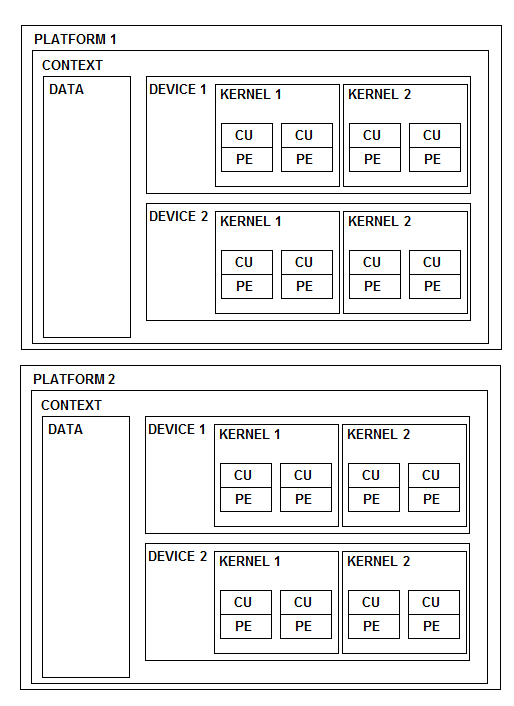
\includegraphics[width=12cm]{rys8}
	\caption{Architektura programu napisanego w bibliotece OpenCL.}
\end{figure}

Pojedyńcza platforma odnosi się do poszczególnego sterownika. Przykładowo na komputerze z procesorem Intel i kartą graficzną AMD mozemy uruchomić dwie platformy, jedną dla OpenCL™ Runtimes for Intel® Processors [https://software.intel.com/en-us/articles/opencl-drivers] i drugą dla wyspecjalizowanego sterownika AMD dla danej karty graficznej. Każda platforma może obsługiwać więcej niż jedno urządzenie, w szczególnych przypadkach może zawierać złożone układy kart graficznych.

\subsection{Urzadzenia OpenCL}\label{sec:OpenC21L}

Standard OpenCL udostępnia 5 różnych rodzajów urządzeń:

- CL_DEVICE_TYPE_CPU - 

\subsection{Kontekst obliczeniowy}\label{sec:OpenC2L}


\subsection{Jednostki obliczeniowe i elementy przetwarzania}\label{sec:OpenC3L}
\subsection{Kernel}\label{sec:OpenC4L}
\subsection{Przestrzen indeksowania}\label{sec:OpenC5L}
Jednostki obliczeniowe i elementy przetwarzania reprezentują różne fizyczne elementy procesora w zależności od jego rodzaju. Dla procesorów CPU CU jest równoważne PE i stanowi pojedyńczy rdzeń procesora. W kartach graficznych NVIDIA CU stanowi multiprocesor strumieniowy, a PE jego rdzenie. Karty graficzne AMD definiują CU jako jednostkę SIMD (ang. Single instruction, multiple thread), a PE jako poszczególne linie jednostki SIMD. Elementy przetwarzania wykonują specjalnie przygotowane funkcje (tzw. kernele), definiowane według standardu OpenCL. Mimo że w zależności od urządzenia CU i PE reprezentują różne elementy procesora, odwołują się do nich w ten sam sposób. Umożliwia to wykonywanie  kernela o jednakowej składni na różnych typach procesorów. Kernele wykonywane są według kolejki zadań i rozdzielone pomiędzy jednostki obliczeniowe mogą być wykonywane równolegle na wielu elementach przetwarzania. Każda kolejka zadań definiuje przestrzeń indeksowania, w której wykonywane są poszczególne kernele.  Instancje kernela wywołaną w obrębie jednego indeksu nazywamy wątkiem. Przestrzeń indeksów można podzielić na grupy (ang. work-group), do których należą poszczególne wątki.

\subsection{Dostep do pamieci}\label{sec:OpenC6L}

OpenCL umożliwia dynamiczny dostęp do pamięci urządzeń. Zdefiniowane są cztery typy pamięci:

- pamięć globalna – pamięć dostępna przez wszystkie wątki w obrębie jednego kontekstu

- pamięć stała – pamięć tylko do odczytu, dostępna globalnie

- pamięć lokalna – pamięć dostępna w obrębie jednej grupy wątków

- pamięć prywatna – pamięć dostępna w obrębie jednego wątku\\


 Przepływ danych między platformą  a urządzeniem może odbyć się poprzez operację kopiowania  lub odwzorowania z pamięci platformy do pamięci urządzenia.

Dużym ograniczeniem wydajności obliczeń jest czas dostępu do pamięci. Pamięć o szerszym zakresie ma wolniejszy czas dostępu, dlatego najwydajniejsze obliczeniawykonują się dla niezależnych wątków działających równolegle o prywatnej pamięci.















